% In this section outline your results. At this point, you are just stating the outcome of your analysis. 
% You can highlight important aspects (``we observe a significantly higher value of $x$ over $y$''), 
% but leave interpretation and opinion to the next section. This section absoultely \emph{has} to include at least two figures.

To model the death rate of ischemic heart disease we tried using a linear model with different transformations of the data, but the results were not satisfactory.
Because of this, we decided to use random forest regression. 
We used the \texttt{RandomForestRegressor} from the \texttt{scikit-learn} library \citep{scikit-learn} with grid search to find the best parameters. 
\begin{figure}[ht]
    \vskip 0.2in
    \begin{center}
    \centerline{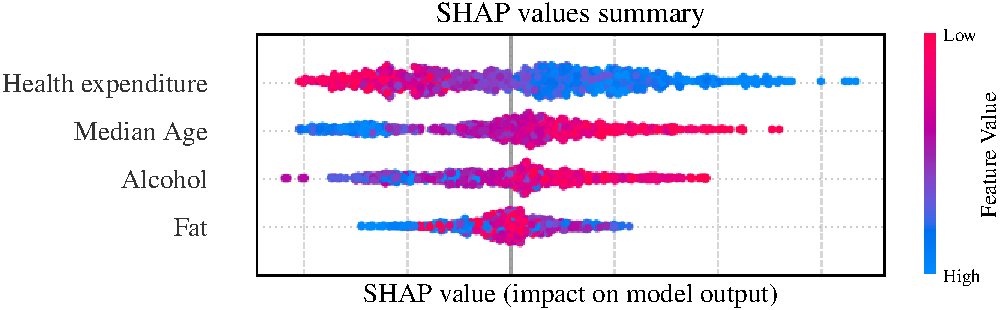
\includegraphics[width=\columnwidth]{fig/fig_shap_values_summary.pdf}}
    \caption{Summary of SHAP values for a predictive model of disease death rate. 
    Each dot's color represents the feature's value, and its position represents the impact on the model's output.}
    \label{shap_values}
    \end{center}
    \vskip -0.2in
\end{figure}
\begin{figure*}[ht]
    \vskip 0.2in
    \centering
    \centerline{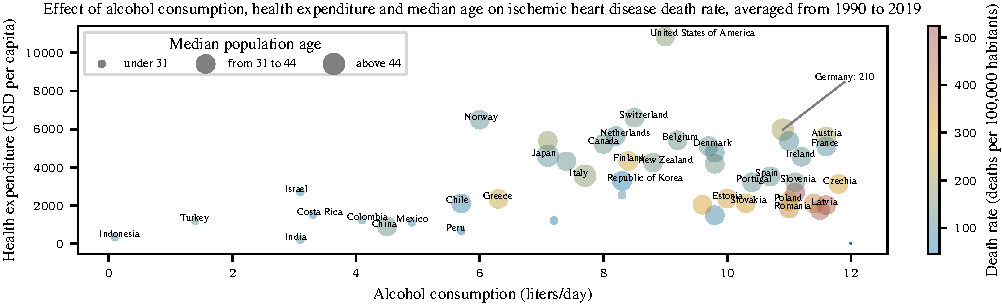
\includegraphics[]{fig/fig_bubble_plot_factors.pdf}}
    \caption{The combined effect of healthcare spending, alcohol consumption, and median age on the death rate of ischemic heart disease. Special 
        emphasis to the comparison between Germany, high income countries, and the world.}
    \label{bubble_plot_factors}
\end{figure*}
Our best model had the 
$R^2$ score of $\approx0.82$ on the test set, while the $R^2$ score of the linear model was $\approx0.39$. The value represents the proportion of the variance that 
is explained by the model. We interpret the model using the SHAP (SHapley Additive exPlanations) values \citep{NIPS2017_7062} (see Figure \ref{shap_values}). SHAP values 
show how the impact of a feature on the model's output. 






We can see that the effect of fat consumption is mixed and not very easy to interpret. The effect of the other three features 
(Healthcare spending, alcohol consumption, and median age) is more clear. For that reason, we decided to use only those three features in our final plot 
(see Figure \ref{bubble_plot_factors}) in which we show the combined effect of the three features on the death rate. The median age is divided into three groups, under 19, 19-38, and over 38. The size of the bubble represents the age group. The position of the bubble represents the healthcare spending and the alcohol consumption. The color represents the death rate from ischemic heart diseases.
Counries with higher alcohol consumption (on the right) appear to have higher death rates.
Larger bubbles (older populations) and bubbles on the right (higher alcohol consumption) appear to have higher death rates, which is consistent with the SHAP values.

